\subsection{Rulebase Plug-in Projekt}

Um ein Rulebase Plug-in Projekt zu erstellen importieren sie am besten ein bestehendes Rulebase Plug-in Projekt (z.B. \texttt{org.sidiff.ecore.recognitionrules.atomic}): File $\triangleright$ Import $\triangleright$ Plug-Ins and Fragments $\triangleright$ Projects with source folders.\\
Anschließend passen Sie den Projektnamen und weitere projektspezifische Bezeichner an Ihre Bedürfnisse an. Exisitierende Rulebases können Sie aus dem Projekt löschen. Verfahren Sie anschließend gemäß Abschnitt \ref{sec:rbfile} mit dem eigentlichen Erzeugen der neuen Erkennungsregeln und des sog. Rulebase-Files.\\


Gehen Sie auf \texttt{File} $\triangleright$ \texttt{New} $\triangleright$ \texttt{Other...} und wählen Sie \texttt{SiLift} $\triangleright$ \texttt{Rulebase Plug-in Project} aus (vgl. Abb. \ref{silift-wizard_rulebase_page01}).
 
\begin{figure}[H]
\centering
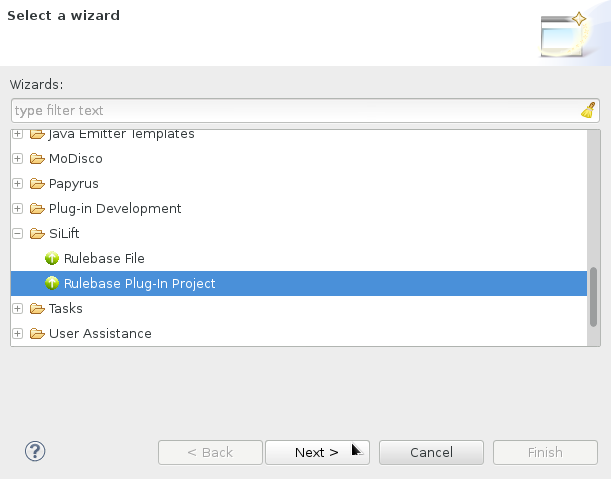
\includegraphics[width=0.6\textwidth]{recognitionrules/graphics/silift-wizard_rulebase_page01.png}
\caption{Erstellen eines \textit{Rulebase Plug-in Projects}}
\label{silift-wizard_rulebase_page01}
\end{figure}

Klicken Sie auf \texttt{Next} und geben Sie einen Projektnamen ein (vgl. Abb. \ref{silift-wizard_rulebase_page02}).

\begin{figure}[H]
\centering
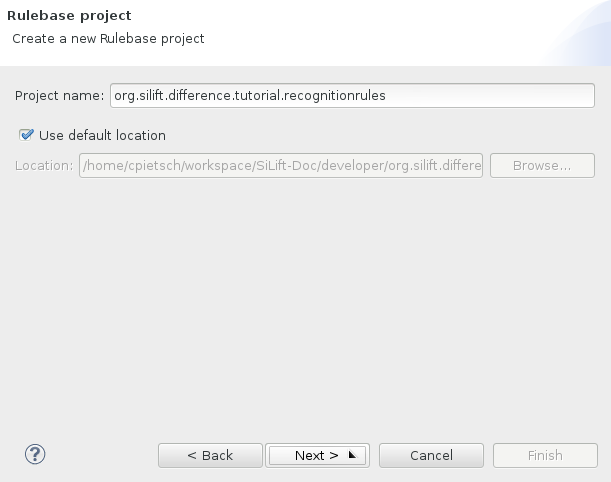
\includegraphics[width=0.6\textwidth]{recognitionrules/graphics/silift-wizard_rulebase_page02.png}
\caption{Erstellen eines \textit{Rulebase Plug-in Projects}}
\label{silift-wizard_rulebase_page02}
\end{figure}

Danach müssen noch die Editierregeln ausgewählt und unter einem entsprechenden Namen abgespeichert werden (vgl. Abb. \ref{silift-wizard_rulebase_page03}).
SiLift erzeugt nun die Erkennungsregeln und speichert diese in einer \textit{Rulebase}.

\begin{figure}[H]
\centering
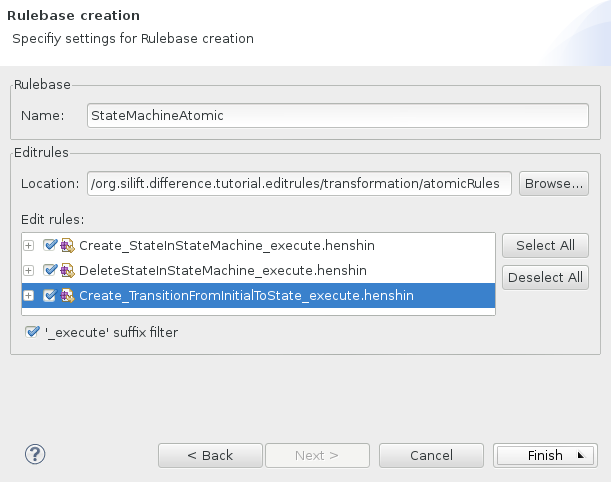
\includegraphics[width=0.6\textwidth]{recognitionrules/graphics/silift-wizard_rulebase_page03.png}
\caption{Erstellen eines \textit{Rulebase Plug-in Projects}}
\label{silift-wizard_rulebase_page03}
\end{figure}

